
\de{ĐỀ THI HỌC KỲ I NĂM HỌC 2022-2023}{THPT Marie Curie}


%-----Câu 1
\begin{bt}
	Tìm tập xác định của hàm số $f(x)=\dfrac{x^2-\sqrt{x-2}}{x^2-5x+6}$.
	\loigiai{
		Hàm số xác định khi và chỉ khi
		\[
		\heva{& x-2\geq 0 \\ & x^2-5x+6\neq0}\Leftrightarrow\heva{& x\geq2 \\ & x\neq2 \\& x\neq 3}\Leftrightarrow\heva{& x>2 \\ & x\neq3.}
		\]
		Vậy $\mathscr{D}=(2;+\infty)\setminus\{3\}$.}
\end{bt} 

%-----Câu 2
\begin{bt}
	Cho hàm số $y=f(x)$ xác định trên đoạn $[-1;5]$ và có đồ thị như hình vẽ.
	\begin{center}\begin{tikzpicture}[>=stealth,x=1cm,y=1cm,scale=1]
			\draw[->](-1.8,0)--(-1,0)node[below]{$-1$}--(1,0)node[below]{$1$}--(2,0)node[below]{$2$}--(3,0)node[below]{$3$}--(4,0)node[above]{$4$}--(5,0)node[above]{$5$}--(5.8,0)node[above]{$x$};
			\draw[->] (0,-1.8)--(0,-1)node[left]{$-1$}--(0,1)node[right]{$1$}--(0,2)node[left]{$2$}--(0,3.2)node[right]{$y$};
			\draw (0,0)node[above left]{$O$};
			\fill[dashed] (-1,1)circle(2pt) edge (-1,0) edge (0,1) (2,2) circle edge (2,0) edge(0,2) (5,-1) circle edge (5,0) edge(0,-1) (-1,0)circle (1pt) (1,0)circle (1pt) (2,0)circle (1pt) (3,0)circle (1pt) (4,0)circle (1pt) (5,0)circle (1pt);
			\clip (-2,-2)rectangle(6,3.5);
			\draw[thick,samples=150,smooth] (-1,1)--(1,0)--(2,2);
			\draw[thick,samples=150,smooth]
			(2,2)..controls+(-20:1)and+(135:0.25)..(3.6,0)
			..controls+(-45:1)and+(155:1)..(5,-1)
			;
		\end{tikzpicture}
	\end{center}
	Hãy xác định các khoảng đồng biến, nghịch biến của hàm số $y=f(x)$ trên khoảng $(-1;5)$.
	\loigiai{
		Hàm số đồng biến trên $(1;2)$, hàm số nghịch biến trên các khoảng $(-1;1)$ và $(2;5)$.
	}
\end{bt}


%-----Câu 3
\begin{bt}
	Cho hàm số $f(x)=\heva{\dfrac{2}{x+1} &\quad\text{ khi } x<-1\\3\sqrt{x+4}&\quad\text{ khi }x\geq -1.}$\\
	Tính giá trị của biểu thức $A=f(0)+f(-3)$.
	\loigiai{
		$A=3\sqrt{0+4}+\dfrac{2}{-3+1}=3\cdot2+(-1)=6-1=5$.
	}
\end{bt}


%-----Câu 4
\begin{bt}
	Cho hàm số $f(x)=ax^2+2x+c$ với $a\neq 0$ có đồ thị $(P)$ như hình vẽ bên.
	\immini{
		\begin{listEX}
			\item Xác định dấu của $a$.
			\item Xác định trục đối xứng của đồ thị $(P)$.
			\item Tìm giao điểm của $(P)$ với hai trục tọa độ.
			\item Lập bảng biến thiên của hàm số.
			\item Tính giá trị $T=f(2)-f(-4)$.
		\end{listEX}
	}{
		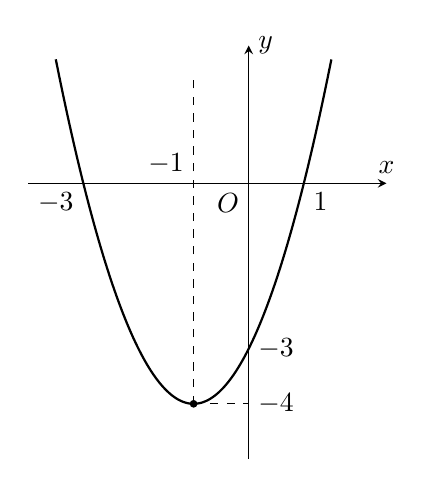
\begin{tikzpicture}[>=stealth,x=1cm,y=1cm,scale=0.7]
			\draw[->](-4,0)--(-3,0)node[below left]{$-3$}--(-1,0)node[above left]{$-1$}--(1,0)node[below right]{$1$}--(2.5,0)node[above]{$x$};
			\draw[->] (0,-5)--(0,-4)node[right]{$-4$}--(0,-3)node[right]{$-3$}--(0,2.5)node[right]{$y$};
			\draw (0,0)node[below left]{$O$};
			\fill[dashed] (-1,-4) circle(2pt) edge (-1,2) edge (0,-4);
			\clip (-4,-5)rectangle(2.5,2.5);
			\draw[thick,samples=150,smooth,domain=-3.5:1.5] plot(\x,{(\x)^2+2*(\x)-3});
		\end{tikzpicture}
	}
	\loigiai{
		\begin{enumerate}
			\item Vì đồ thị $f(x)$ có bề lõm hướng lên trên nên $a>0$.
			\item $x=-1$.
			\item $A(0,-3)$, $B(-3,0)$ và $C(1,0)$.
			\item Bảng biến thiên
			\begin{center}
				\begin{tikzpicture}[yscale=.8,xscale=1.2]
					\def\a{6} % số cột nhãn
					\def\b{2} % số hàng nhãn
					%\pagecolor{yellow!30}
					\draw[shift={(-.5,.5)}]
					%	(-1.5,0.25) rectangle (\a,-\b-.25)
					(-1.5,-1)--+(0:\a+1)
					%	(-1,-2)--+(0:\a+1)
					%	(-1,-3)--+(0:\a+1)
					(1,0)--+(-90:\b)
					;
					\path
					(-.75,0) node {$x$}
					(-.85,-1) node {$ax^2 + 2x +c$}
					(1.25,-1) node {$-$}
					%(1,-2) node {$+$}
					%(1,-3) node {$-$}
					%(2,0.1) node {$\dfrac{3}{7}$}
					%(2,-1) node {$0$}
					(2.5,0) node {$-1$}
					(2.5,-1) node {$0$}
					%(3,-2) node {$+$}
					%(3,-3) node {$+$}
					%(4,0) node {$1$}
					%(4,-1) node {$0$}
					%(4,-3) node {$0$}
					(4,-1) node {$+$}
					%(5,-2) node {$-$}
					%(5,-3) node {$-$}
					;
				\end{tikzpicture}
			\end{center}
			\item Thay $x=-3$ và $y=0$ vào $f(x)$, ta có $9a-6+c=0\Leftrightarrow9a+c=6$.\hfill$(1)$\\
			Thay $x=1$ và $y=0$ vào $f(x)$, ta có $a+2+c=0\Leftrightarrow a+c=-2$.\hfill$(2)$\\
			Từ $(1)$ và $(2)$ ta có hệ phương trình $\heva{& 9a+c=6 \\ & a+c=-2}\Leftrightarrow\heva{& a=1 \\ & c=-3.}$\\
			Vậy $f(x)=x^2+2x-3$, ta có
			\[
			T=f(2)-f(-4)=2^2+2\cdot2-3-(-4)^2-2\cdot(-4)+3=4+4-3-16+8+3=0.
			\]
		\end{enumerate}
	}
\end{bt}

%-----Câu 5
\begin{bt}%[0T6B3-1]%[0T6B3-2]%[0T6B3-3]
Tuổi thọ của $30$ bóng đèn thắp thử (đơn vị giờ) được cho bởi bảng số liệu thống kê dưới đây
\begin{center}\begin{tabular}{|cccccccccc|}
\hline
$1180$ & $1150$ & $1190$ & $1170$ & $1180$ & $1170$ & $1160$ & $1170$ & $1160$ & $1150$ \\
$1190$ & $1180$ & $1170$ & $1170$ & $1170$ & $1190$ & $1170$ & $1170$ & $1170$ & $1180$
 \\
$1170$ & $1160$ & $1160$ & $1160$ & $1170$ & $1160$ & $1180$ & $1180$ & $1150$ & $1170$ 
 \\
\hline
\end{tabular}
\end{center}
\begin{listEX}
\item Lập bảng phân bố tần số.
\item Tính số trung bình của mẫu số liệu trên.
\item Tính mốt và trung vị của mẫu số liệu.
\end{listEX}
\loigiai{
\begin{enumerate}
\item Bảng phân bố tần số
\begin{center}
	\begin{tabular}{|c|c|c|c|c|c|c|}
		\hline 
		Giá trị $(x)$&$1150$&$1160$&$1170$&$1180$&$1190$&\\
		\hline 
		Tần số $(n)$&$3$&$6$&$12$&$6$&$3$&$N=30$\\
		\hline	
	\end{tabular}
\end{center}
\item Trung bình cộng của mẫu số liệu trên là
\[\overline{x}=\dfrac{1150\cdot 3+1160\cdot 6+1170\cdot 12+1180\cdot 6+1190\cdot 3}{30}=1170.\]
\item Mốt của mẫu số liệu là $M_o=1170$.\\
Trung vị của mẫu số liệu là $M_e=\dfrac{1170+1170}{2}=1170$.
\end{enumerate}
}
\end{bt}

%-----Câu 6
\begin{bt}%[0T5B3-1]%[0T5B4-1]%[0T5B3-4]%[Dự án Đề kiểm tra HKIi NH22-23-TinDatTran]%[THPT Marie Curie]
Cho hình vuông $ABCD$ tâm $O$ có $AB=3$.
\begin{listEX}[2]
\item Tính $\overrightarrow{BO}\cdot \overrightarrow{BC}$
\item Tính $\left|\overrightarrow{AO}+\overrightarrow{AB}\right|$.
\item* Gọi $M$ là điểm trên cạnh $CD$ thỏa mãn $MD=2MC$ và $N$ là trung điểm của $AM$. Hãy phân tích véc-tơ $\overrightarrow{DN}$ theo hai véc-tơ $\overrightarrow{AC}$ và $\overrightarrow{BC}$.
\end{listEX}
\loigiai{
\begin{enumerate}
\item 
\immini{
Ta có 
\begin{align*} 
\overrightarrow{B O} \cdot \overrightarrow{B C} & =\overrightarrow{B O}(\overrightarrow{B O}+\overrightarrow{O C}) \\ 
& =B O^2+\overrightarrow{B O} \cdot \overrightarrow{O C} \\ 
& =\left(\frac{B D}{2}\right)^2+0 \\ & =\left(\frac{3 \sqrt{2}}{2}\right)^2=\frac{9}{2}
\end{align*}}
{
\begin{tikzpicture}
\def\c{4}
\path 
(0,\c) coordinate (A)
(\c,0) coordinate (C)
(0,0) coordinate (D)
($(A)+(C)-(D)$) coordinate (B)
($(A)!.5!(C)$) coordinate (O)
($(B)!0.5!(O)$) coordinate (I)
($(D)!2/3!(C)$) coordinate (M)
($(A)!.5!(M)$) coordinate (N)
;
\draw (A)--(B)--(C)--(D)--cycle (A)--(M) (D)--(B) (A)--(C) (D)--(N);
\foreach \x/\y in {A/145,B/45,C/-135,D/-45,O/0,I/90,M/-90,N/180}{\fill (\x) circle(1pt)node[shift={(\y:.35)}]{$\x$};}
\end{tikzpicture}
}
\item Gọi $I$ là trung điểm của $BO$.\\
Ta có 
\begin{align*}
	\left|\overrightarrow{A O}+\overrightarrow{A B}\right|&=\left|2 \overrightarrow{A I}\right|=2 A I \\
	&=2 \sqrt{A O^2+O I^2}\\
	&=2 \sqrt{A O^2+\left(\frac{A O}{2}\right)^2}\\
	&=2 \sqrt{\left(\frac{3 \sqrt{2}}{2}\right)^2+\left(\frac{3 \sqrt{2}}{4}\right)^2} \\
	&=\frac{3 \sqrt{10}}{2}.
\end{align*}
\item
Do $N$ là trung điểm của $AM$ nên ta có
\begin{align*}
	\overrightarrow{D N}&=\frac{1}{2}(\overrightarrow{D A}+\overrightarrow{D M}) =\frac{1}{2}\left(-\overrightarrow{B C}+\frac{2}{3} \overrightarrow{D C}\right)=-\frac{1}{2} \overrightarrow{B C}+\frac{1}{3} \overrightarrow{A B} \\
	&=-\frac{5}{6} \overrightarrow{B C}+\frac{1}{3} \overrightarrow{A B}+\frac{1}{3} \overrightarrow{B C}=-\frac{5}{6} \overrightarrow{B C}+\frac{1}{3} \overrightarrow{A C}.
\end{align*}
\end{enumerate}
}
\end{bt}

%-----Câu 7
\begin{bt}%[0T2B2-1]
Biểu diễn miền nghiệm của hệ bất phương trình $\heva{&x\geq 0\\&y\leq 0\\&2x-3y-6\leq 0.}$
\loigiai{
\immini{
Trên mặt phẳng $Oxy$ vẽ đường thẳng $\Delta\colon 2 x-3 y-6=0$ đi qua các điểm $A(0;-2)$, $B(3;0)$.\\
Chọn $O(0 ; 0) \notin \Delta$.\\
Vì $2\cdot0-3\cdot0-6=-6<0$ nên miền nghiệm của
bất phương trình $2 x-3 y-6 \leq 0$ là nửa mặt phẳng bờ $\Delta$ chứa $O$ và kể cả bờ $\Delta$.\\
Vậy miền nghiệm của hệ bất phương trình trên là $\triangle O A B$ (kể cả bờ) với $A(0 ;-2)$ và $B(3 ; 0)$.}
{\begin{tikzpicture}[>=stealth,smooth,samples=100,font=\scriptsize]
		\begin{scope}
						\clip (-1,-3) rectangle (4,2);
			\draw[->] (-4,0)--(4,0);
			\draw[->] (0,-4)--(0,4);

			\foreach \i in {-11,-10.85,...,11}{
				\draw[thin,teal!65](0,{\i})--+(130:10);}
			\draw[variable=\t] plot[domain=-11:11]({-(0)},{\t});
			\foreach \i in {-11,-10.85,...,11}{
				\draw[teal!65,thin]({\i},{(-0*\i-0)/1})--+(60:10);}
			\draw plot[domain=-9:9]({\x},{(-0*\x-0)/1});
			\foreach \i in {-11,-10.85,...,11}{
				\draw[teal!65,thin]({\i},{(-2*\i--6)/-3})--+(-60:10);}
			\draw plot[domain=-9:9]({\x},{(-2*\x--6)/-3});
			\path (A)--(B) node[above=-2pt,pos=0.5,sloped,rectangle,rounded corners,fill=white]{$\tiny\Delta\colon2x-3y-6 = 0$};
		\end{scope}
		\path (0,-2) coordinate (A)
		(3,0) coordinate (B)
		(0,0) coordinate (O);
		\draw[thick](A)--(O)--(B)--cycle;
		\foreach \x/\y in {A/60,B/-160,O/-45}{\fill (\x) circle(1pt)node[shift={(\y:.4)}]{$\x$};}
\end{tikzpicture}}
}
\end{bt}


